\newpage
\subsubsection{Join}
Specifying two (or more) tables in the \texttt{FROM} clause will perform a cartesian product, e.g.
\mint{sql}|SELECT * FROM (Table1, Table2);|
returns all rows of the tables, next to each other.

Here, naming the tables in the \texttt{FROM} clause may come in handy, to not write out the entire name of the tables:
\mint{sql}|SELECT * FROM (Table1 t, Table2 s) WHERE t.id = s.id;|
\mint{sql}|SELECT * FROM (Table1, Table2) WHERE Table1.id = Table2.id;|
Both of the above statements produce the same result.


\paragraph{Nested Queries}
\label{sec:nested-queries}
To not have the cartesian product executed in the \texttt{FROM} clause, or to get a much more complex starting table, we can use a \gls{subquery}.
These are parenthesized normal SQL queries.

We can create an alias for them using an \texttt{AS name} clause after the parenthesis as follows
\mint{sql}|SELECT r.name FROM (SELECT * FROM Table) AS r;|
or alternatively, using a \texttt{WITH} clause (replace the dummy queries with real queries):
\mint{sql}|WITH CteName (SELECT * FROM Table) SELECT name FROM CteName;|


\paragraph{Join Operations}
If we don't specify the kind of join, an \texttt{INNER JOIN} is executed. The following three queries are equivalent
\mint{sql}|SELECT * FROM Student, Tests WHERE Student.PersNr = Tests.PersNr;|
\mint{sql}|SELECT * FROM Student JOIN Tests ON Student.PersNr = Tests.PersNr;|
\mint{sql}|SELECT * FROM Student JOIN Tests USING (PersNr);|
For the latter of the three, the parenthesis around the column are important, as omitting them is invalid syntax.

Other types of \texttt{JOIN} are:
\begin{itemize}
    \item \texttt{NATURAL JOIN} (no \texttt{ON} required), joins on columns with same name
    \item \texttt{LEFT/RIGHT/FULL OUTER JOIN} (requires \texttt{ON}), also returns non-matching rows from left, right or both sides, respectively
\end{itemize}

\begin{center}
    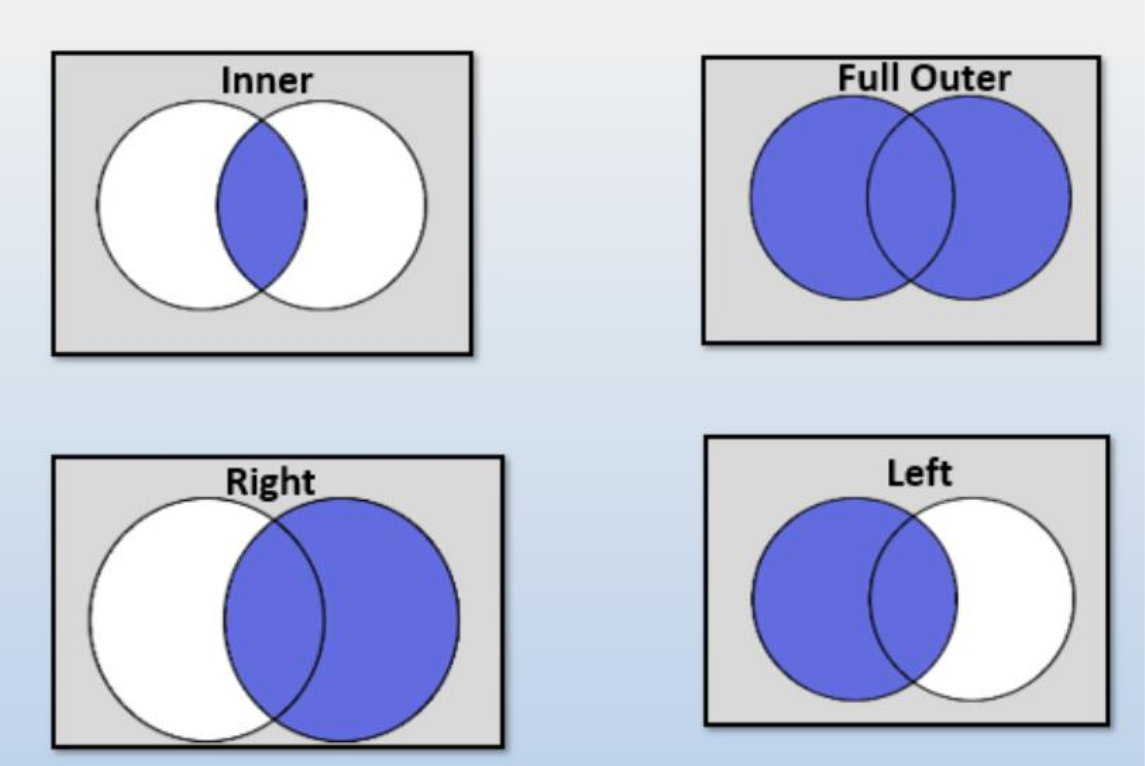
\includegraphics[width=0.5\textwidth]{assets/join-types.png}
\end{center}
